\Class{Templar}
{Against the law? The law is a convenience, a tool for us to use as we will, not a yoke bound to our necks. Laws are guidelines, not rules cast in iron. Stretching them is not the same as breaking them, my young apprentice. Take that to heart, for if you accuse me again, I will have your heart served cold.}{Zelgado De'Draigee, human templar}

Templars are civil servants within a city-state's government organization commonly referred to as a ``temple,'' ``bureau,'' or ``order.'' Each templar swears obedience to his temple, and absolute fealty to his sorcerer-king. In return, the sorcerer-king grants them spell power stolen from the elemental planes.

In most city-states, templars are the ultimate authority---judge, jury, and executioner. Templars police and administer the city-states, and serve other civil roles ranging from general to jailor and from tax collector to garbage collector.

\SpellcasterTable{The Templar}{.4cm}{
1 & +0 & +2 & +0 & +2 & Secular aptitude, assume domain, sigil & 5 & 3+1 &&&&&&&&\\
2 & +1 & +3 & +0 & +3 && 6 & 4+1 &&&&&&&&\\
3 & +2 & +3 & +1 & +3 && 6 & 5+1 &&&&&&&&\\
4 & +3 & +4 & +1 & +4 & Turn or rebuke undead & 6 & 6+1 & 3+1 &&&&&&&\\
5 & +3 & +4 & +1 & +4 && 6 & 6+1 & 4+1 &&&&&&&\\
6 & +4 & +5 & +2 & +5 & \feat{Scribe Scroll} & 6 & 6+1 & 5+1 & 3+1 &&&&&&\\
7 & +5 & +5 & +2 & +5 && 6 & 6+1 & 6+1 & 4+1 &&&&&&\\
8 & +6/+1 & +6 & +2 & +6 & \feat{Brew Potion} & 6 & 6+1 & 6+1 & 5+1 & 3+1 &&&&&\\
9 & +6/+1 & +6 & +3 & +6 && 6 & 6+1 & 6+1 & 6+1 & 4+1 &&&&&\\
10 & +7/+2 & +7 & +3 & +7 && 6 & 6+1 & 6+1 & 6+1 & 5+1 & 3+1 &&&&\\
11 & +8/+3 & +7 & +3 & +7 && 6 & 6+1 & 6+1 & 6+1 & 6+1 & 4+1 &&&&\\
12 & +9/+4 & +8 & +4 & +8 && 6 & 6+1 & 6+1 & 6+1 & 6+1 & 5+1 & 3+1 &&&\\
13 & +9/+4 & +8 & +4 & +8 && 6 & 6+1 & 6+1 & 6+1 & 6+1 & 6+1 & 4+1 &&&\\
14 & +10/+5 & +9 & +4 & +9 && 6 & 6+1 & 6+1 & 6+1 & 6+1 & 6+1 & 5+1 & 3+1 &&\\
15 & +11/+6/+1 & +9 & +5 & +9 && 6 & 6+1 & 6+1 & 6+1 & 6+1 & 6+1 & 6+1 & 4+1 &&\\
16 & +12/+7/+2 & +10 & +5 & +10 && 6 & 6+1 & 6+1 & 6+1 & 6+1 & 6+1 & 6+1 & 5+1 & 3+1 &\\
17 & +12/+7/+2 & +10 & +5 & +10 && 6 & 6+1 & 6+1 & 6+1 & 6+1 & 6+1 & 6+1 & 6+1 & 4+1 &\\
18 & +13/+8/+3 & +11 & +6 & +11 && 6 & 6+1 & 6+1 & 6+1 & 6+1 & 6+1 & 6+1 & 6+1 & 5+1 & 3+1 \\
19 & +14/+9/+4 & +11 & +6 & +11 && 6 & 6+1 & 6+1 & 6+1 & 6+1 & 6+1 & 6+1 & 6+1 & 6+1 & 4+1 \\
20 & +15/+10/+5 & +12 & +6 & +12 && 6 & 6+1 & 6+1 & 6+1 & 6+1 & 6+1 & 6+1 & 6+1 & 6+1 & 5+1
}
\begin{figure}[t!]
\centering
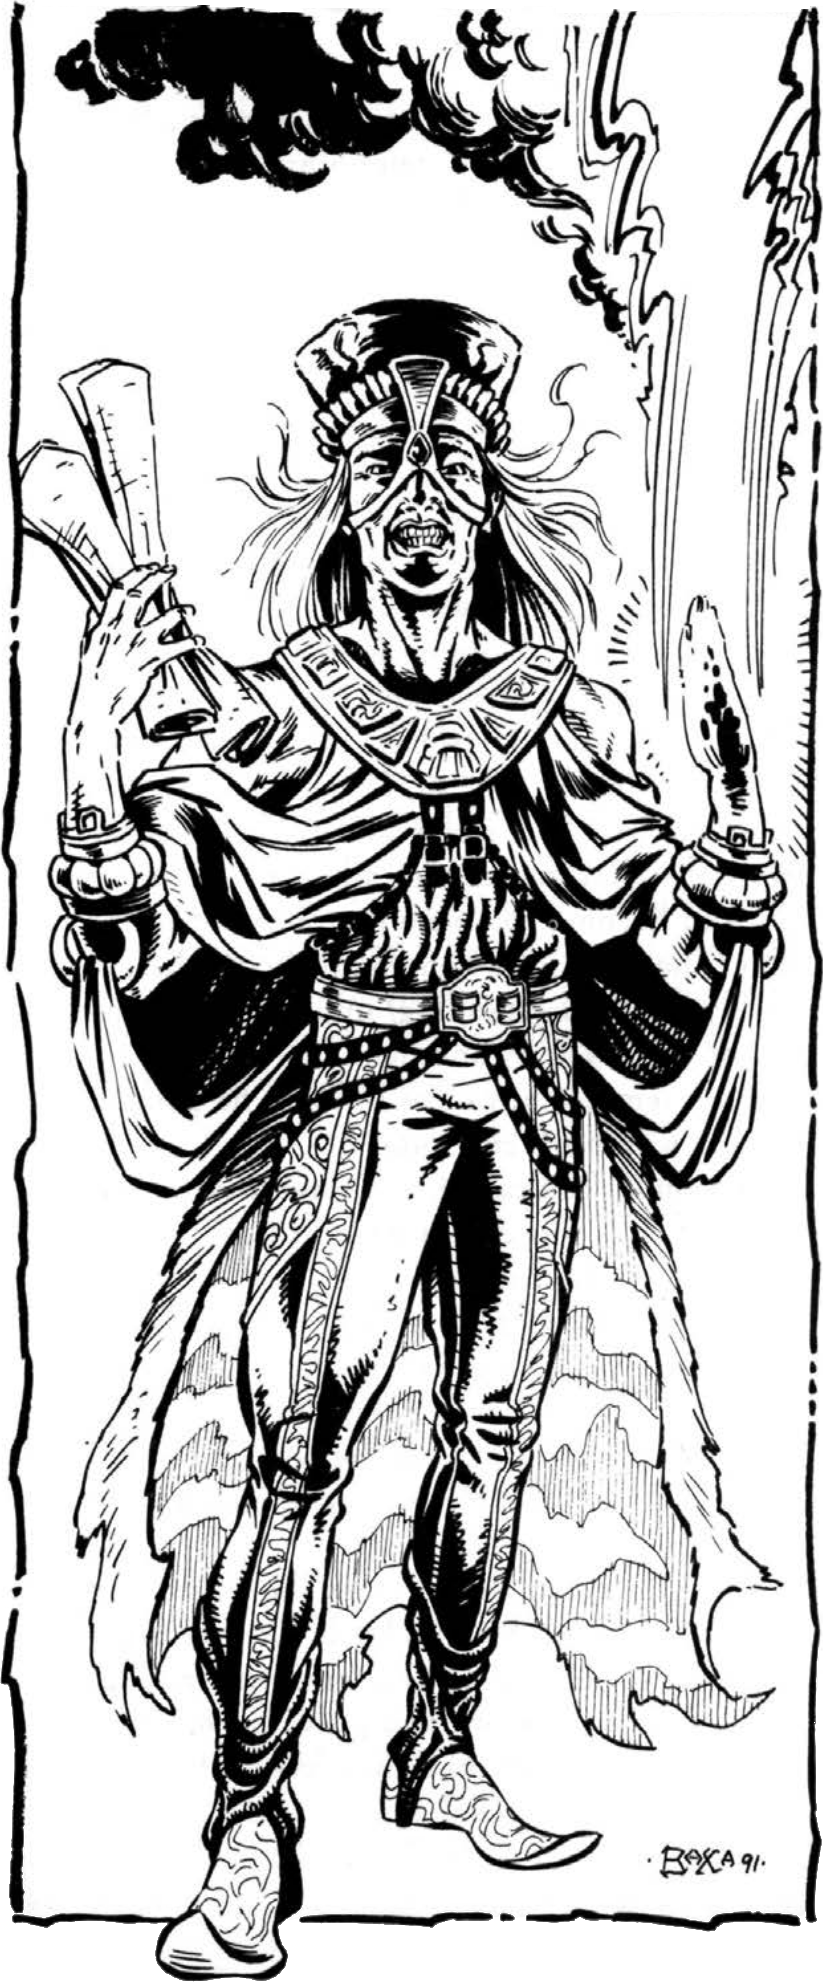
\includegraphics[width=\columnwidth]{images/templar-1.png}
\WOTC
\end{figure}

\subsection{Making a Templar}
Templars can cast a number of divine spells each day, as granted by their lord. If necessary they can be a destructive fighting force, but they serve much better as officers of slave-soldiers, mercenaries, or undead. Their wide array of available skills reflects the equally wide array of roles that Templars fill as servants of the sorcerer-kings and queens.

\textbf{Abilities:} If you want to make good use of your templar spells and you secular aptitude, you'll need a high Charisma. As with any melee-oriented class, Strength is a key ability for templars and Constitution provides you with increased ht points as usual.

\textbf{Races:} While the need for religion and divine magic is nearly universal on Athas, the need for specialized militant priest--bureaucrats is peculiar to large city-states dominated by sorcerer-kings. While in theory, no sentient race is precluded from the templar class, in practice, a sorcerer-king grant spells only to those who he wants to represent him. Humans dominate the templar priesthoods of all city-states except for New Giustenal. Dwarves, muls, and half-elves commonly become templars in many cities, while elves are less commonly accepted. Templars of other races are rare or unheard--of in most cities.

\textbf{Alignment:} A templar's alignment must be within one step of his sorcerer-king's (that is, it may be one step away on either the lawful--chaotic axis or the good--evil axis, but not both). Because of that, templars are almost never good. The laws they uphold are corrupt; the monarchs they serve are arguably the vilest creatures on the face of Athas, and often the templars are cruel and unjust themselves. However, many templars take considerable pride in the prosperity and magnificence of their city-state, and in the well--oiled machine of their order. Templars are most commonly lawful neutral or lawful evil.

\subsection{Game Rule Information}

\textbf{Alignment:} A templar's alignment must be within one step of his sorcerer-monarch's in each axis (that is, it may be one step away on the lawful-chaotic axis or the good-evil axis, but not two steps in either of them). A cleric may not be neutral unless his sorcerer-monarch's alignment is also neutral.

\textbf{Hit Die:} d8.

\subsubsection{Class Skills}
\skill{Appraise} (Int), \skill{Bluff} (Cha), \skill{Concentration} (Con), \skill{Craft} (Int), \skill{Diplomacy} (Cha), \skill{Forgery} (Int), \skill{Gather Information} (Cha), \skill{Heal} (Wis), \skill{Intimidate} (Cha), \skill{Knowledge} (all skills individually) (Int), \skill{Literacy} (N/A), \skill{Profession} (Wis), \skill{Sense Motive} (Wis), \skill{Spellcraft} (Int), and \skill{Spot} (Wis).

\textbf{Skill Points per Level:} 4 + Int modifier ($\times 4$ at 1st level).

\subsubsection{Class Features}

\textbf{Weapon and Armor Proficiency:} Templars are proficient in all simple weapons. Since templar training involves some education in warfare, templars receive two martial weapons proficiencies. Templars are proficient in light and medium armor and shields (except tower shields).

\textbf{Spellcasting:} A templar casts divine spells, which are drawn from the templar spell list. When she gain access to a new level of spells, she automatically knows all the spells for that level on the templar's spell list. She can cast any spell she know without preparing it ahead of time. Essentially, her spell list is the same as her spells known list.

To cast a spell, a templar must have a Charisma score of 10 + the spell's level. The Difficulty Class for a saving throw against a templar's spell is 10 + the spell's level + the templar's Cha modifier. Like other spellcasters, a templar can cast only a certain number of spells of each level per day. The base daily allotment is given on \tabref{The Templar}. In addition, she receives bonus spells if she has a high Charisma score.

She can also cast one domain spell of each spell level per day, as a cleric does. The domain spell is chosen at the time of casting from the spells associated with your assumed domains (see below), as she casts spells spontaneously and need not prepare spells ahead of time.

A templar need not prepare spells in advance. She can cast any spell she knows at any time, assuming she has not yet used up your spells per day for that spell level.

Templars use their sorcerer-king's sigil as divine focus.

\textbf{Secular Aptitude (Ex):} A templar gains \feat{Secular Authority} as a bonus feat. In addition, she receives a competence bonus to Secular Authority checks equal to half her class level.

\textbf{Assume Domain:} A templar is assigned two domains based on her sorcerer-monarch. Each domain gives her access to a domain spell at each spell level she can cast, from 1st on up, as well as a granted power. She gets the granted powers of both the assumed domains. With access to two domain spells at a given spell level, she adds only one of those spells to your spells known list.

\Table{Sorcerer-Kings' Domains and Alignment}{l X l}{
\tableheader Sorcerer-Monarch & \tableheader Domains & \tableheader Alignment\\
Abalach-Re & Chaos, Charm & Chaotic Evil \\
Andropinis & Law, Nobility & Neutral Evil \\
Borys & Destruction, Protection & Lawful Evil \\
Daskinor & Chaos, Madness & Lawful Evil \\
Dregoth & Death, Destruction & Chaotic Evil \\
Hamanu & Strength, War$\dagger$ & Neutral Evil \\
Kalak & Magic, Trickery & Neutral Evil \\
Lalali-Puy & Animal, Plant & Neutral Evil \\
Nibenay & Magic, Mind & Neutral Evil \\
Oronis & Knowledge, Protection & Neutral Good \\
Tectuktitlay & Glory, Strength & Neutral Evil \\
\rowcolor{white}
\multicolumn{3}{l}{$\dagger$ Hamanu's favored weapon is the longsword.}
}

\textbf{Sigil (Sp):} Every templar receives a sigil that is the sign of their rank and station as a templar within their city's templarate. The form of the sigil is unique to each city-state, but is always unmistakable for what it is. The sigil serves as your divine focus, and also allows you to use the spell-like powers \spell{arcane mark}, \spell{purify food and drink}, and \spell{slave scent} a combined total of times equal to 3 + your Cha modifier. These spell-like powers do not count against your total of spells per day.

\textbf{Turn or Rebuke Undead (Su):} Any templar, regardless of alignment, has the power to affect undead creatures by channeling the power of his sorcerer-king through his sigil.

A good templar (or a neutral templar who worships a good sorcerer-king) can turn or destroy undead creatures. An evil templar (or a neutral templar who worships an evil sorcerer-king) instead rebukes or commands such creatures. A neutral templar of a neutral sorcerer-king must choose whether his turning ability functions as that of a good templar or an evil templar. Once this choice is made, it cannot be reversed.

A templar may attempt to turn undead a number of times per day equal to 3 + your Charisma modifier. A templar with 5 or more ranks in \skill{Knowledge} (religion) gets a +2 bonus on turning checks against undead. A templar turns undead as a cleric of three levels lower would.

\textbf{Scribe Scroll:} At 6th level, a templar gains \feat{Scribe Scroll} as a bonus feat.

\textbf{Brew Potion:} At 8th level, a templar gains \feat{Brew Potion} as a bonus feat.

\subsubsection{Ex-Templars}
A templar who displeases or abandons his sorcerer-monarch, or one whose sorcerer-monarch dies, loses all templar spellcasting abilities. An ex-templar is treated as a member of an NPC class (commoner, expert, etc) for purposes of determining CR. If the templar later becomes the templar of another sorcerer-monarch, he immediately regains his full templar spellcasting abilities.

\subsection{Playing a Templar}

A templar can take the fighter's place in the front ranks of a party or ensorcel his foes from a distance like a cleric. While you aren't quite as good as either a dedicated fighter or a dedicated cleric or psion in those roles, you're reasonably effective in either, and you can change roles on a round-by-round basis as needed.

As a templar, you believe the acquisition of power and influence is a worthy end in itself. By having power, you can effect your will in the world, be it good or bad. Those who have or seek power deserve your respect, while those who have power but fail to use it deserve your derision.

You adventure out of a desire to gain more power and influence in every quest. Drawn by your power, others follow your lead, and you are happy to command them.

\subsubsection{Religion}
The reverence of templars and their respective sorcerer-monarch varies greatly with the city-state. Some rulers, like Hamanu or Lalali-Puy, claim they are gods and demand their citizen and templars to worship them as such. Other, like Nibenay and Andropinis, only require service, not worship, from their templars.

\subsubsection{Other Classes}
Templars sometimes clash with druids and elemental clerics, who represent an older, more primal relationship between mortal, nature, and the elements. Templars tend to tolerate these ``primitive priests,'' as long as the druids and clerics do not share their opinions that sorcerer-kings are usurpers of profane divine elemental power. Templars get along with most other classes very well, provided of course that a templar is in charge.

\subsubsection{Combat}
Most of a templar's spells target a single target or have a range of touch, so you are most effective when you single out and focus upon defeating a single opponent. Your spells that affect areas are limited mostly to cones,
which means you need to be on or near the front lines to get the greatest effect from them. Even if you come close to being effective as a fighter or cleric in his chosen field, you're certainly not as effective as a fighter and a cleric.

Outside combat, use your secular authority to its greatest advantage, securing troops and resources for when it happens. If you have a cleric or other healer in the group, save your cures for emergency healing, since a cleric can spontaneously convert their spells into healing ones. If no other healer is present, save it to heal yourself and your allies after combat.

\subsubsection{Advancement}
You don't necessarily profit most from remaining a templar throughout your advancement, since you will lose all your spellcasting abilities in case you displease your sorcerer-king, or in the remote possibility your sorcerer-king dies. If you do multiclass, picking an arcane or psionic class is an excellent choice, especially one that has Charisma as a key ability. Alternatively, you might consider beginning your career as either a wizard or as a wilder, then multiclassing into a templar.

Assign as many skill points as possible to Bluff, Diplomacy, and Sense Motive, since these will be helpful in politics even if you are stripped out of your spells. For feats, take the Negotiator feat and also consider metamagic feats, such as Silent Spell and Empower Spell.

\subsection{Starting Packages}
\subsubsection{The Blaster}
Human Templar

\textbf{Ability Scores:} Str 8, Dex 14, Con 13, Int 10, Wis 12, Cha 15.

\textbf{Skills:} \skill{Bluff}, \skill{Concentration}, \skill{Diplomacy}, \skill{Knowledge} (local), \skill{Sense Motive}, \skill{Spellcraft}.

\textbf{Languages:} Common.

\textbf{Feat:} \feat{Combat Casting}, \feat{Weapon Focus} (ranged spell).

\textbf{Weapons:} Macahuitl (1d8/19--20)

Light crossbow with 20 bolts (1d8/19--20, 24 m).

\textbf{Armor:} Leather (+2 AC).

\textbf{Other Gear:} Sigil, standard adventurer's kit, 43 cp.

\subsubsection{The Controller}
Dwarf Templar

\textbf{Ability Scores:} Str 10, Dex 8, Con 14, Int 14, Wis 13, Cha 13.

\textbf{Skills:} \skill{Bluff}, \skill{Diplomacy}, \skill{Intimidate}, \skill{Knowledge} (local), \skill{Sense Motive}.

\textbf{Languages:} Common, Dwarven, Elven, Saurian.

\textbf{Feat:} \skill{Spell Focus} (enchantment).

\textbf{Weapons:} Puchik (1d4/$\times$3)

Light crossbow with 20 bolts (1d8/19--20, 24 m).

\textbf{Armor:} Scale mail (+4 AC).

\textbf{Other Gear:} Sigil, standard adventurer's kit, 34 cp.

\subsubsection{The Politician}
Elf Templar

\textbf{Ability Scores:} Str 8, Dex 14, Con 8, Int 13, Wis 14, Cha 15.

\textbf{Skills:} \skill{Bluff}, \skill{Diplomacy}, \skill{Knowledge} (nobility and royalty), \skill{Literacy}, \skill{Sense Motive}.

\textbf{Languages:} Common, city language, Elven.

\textbf{Feat:} \feat{Negotiator}.

\textbf{Weapons:} Dagger (1d4/19--20, 3 m).

\textbf{Armor:} Leather (+2 AC).

\textbf{Other Gear:} Sigil, standard adventurer's kit, 113 cp.

\subsection{Templars on Athas}
\Quote{Power does not corrupt men. Fools, however, if they get into a position of power, corrupt power.}{Gorg the mad}

Templar duties typically prevent them from adventuring in the standard sense. They often serve missions for their superiors, typically to recover an important item, assassinate a troublemaker, force the hand of a merchant house or barter with an elf tribe. But that is not to say that templars cannot pursue their own interests.

While all templars are technically bound to their civil service positions on a daily basis, a sufficient bribe can buy them a few days of freedom and adventure, as long as they do not get caught going against the interests of their temple or sorcerer-king. Most templars who do adventure, do so for personal power, seeking to acquire items of great power, or for money or fame to impress their lord or superiors.

\subsubsection{Daily Life}
A templar remains ever ready to face the challenges of the Athasian life. Without the need to rest, study or pray for their powers, templars can leap up in pursuit of whatever their templarate requires them to do.

Templars often possess the charisma and take-charge attitude required of great leaders, but many suffer from an inability to empathize with those they lead. Templars respect the pursuit of might and its use, and they often minimize the value of those who adhere to other philosophies. Even among themselves, templars tend to be contentious, battling for power over the cost of another one.

\subsubsection{Notables}
Living in the shadow of their sorcerer-king, templars who develop too much power and influence are usually executed without a second thought. Nonetheless, there are a few who manage to hide their powers and postpone this unavoidable fate. The most famous templar of the Tyr Region managed to do what was thought to be impossible: succeed the throne of a sorcerer-king. Tithian of Mericles helped in the assassination plot to kill King Kalak of Tyr and in return was put into the throne by Agis of Asticles and his allies.

\subsubsection{Organizations}
While not all templars are members of the same bureau or even the same city-state, they all have the same basic organization. These organizations vary dramatically from one place to the other, however. The city-state of Kurn, for instance, only employs those who genuinely wish to protect and serve the people, whereas the members from Eldaarich are chosen only from the most brutal, cruel, and vicious members from the templar's families.

Regardless, a templar's daily life allows little free time. Waking hours not spent in direct service to the templarate, on patrol, or on the field of battle are filled with martial training, divine study, and bureaucratic
activities.

\subsubsection{NPC Reactions}
Templars who do not show affiliation with their city-state's templarate rarely elicit an unusual reaction from others. To most they might seem as a fighter or perhaps a cleric. Those who know or their connection or see evidence of it, such as their sigil or typical clothing react depending on their attitude toward the templar's sorcerer-king (or bureau). This reaction is one step closer to hostile if the sorcerer-monarch is feared or hated by that individual (which is the most likely scenario). The reaction is one step closer to friendly if that individual is directly associated with that sorcerer-monarch. Clerics, druids, and others who are deeply entrenched with a moral outlook view the templar's choice with great suspicion, and their reaction is one step closer to hostile regardless of the templar's sorcerer-monarch.

\subsubsection{Templar Lore}
Characters with ranks in \skill{Knowledge} (local) can research templars to learn more about them. When a character makes a skill check, read or paraphrase the following, including the information from lower DCs.

\textbf{DC 10:} Templars are the minions of the sorcerer-kings and can draw mystical energies from them.

\textbf{DC 15:} A templar dedicates himself to a particular sorcerer-monarch and gains powers based on the sorcerer-monarch chosen. They can control undead, cast divine spells and have control over the city's resources.

\textbf{DC 20:} In addition to the details above, the result allows the PC to know that a templar has a similar connection to their sorcerer-monarch like a cleric and his element, and if that particular sorcerer-monarch dies, the connection is lost and the templar loses all his powers.